\chapter{Artificial intteligence}

\section{Self-awareness}
    \noindent
    \textbf{Self-awareness} means the ability of a being to know that ``I am experiencing'' and the ability to think about its own states, actions, and continuity over time.
    
    \medskip
    \noindent
    In short, its main aspects are:
    \begin{itemize}
        \item \textbf{Bodily/sensory awareness}: being aware of pain, heat, or body position.
        \item \textbf{Reflective awareness}: making your experience the subject of thought (``I was scared because there was a loud noise'').
        \item \textbf{Temporal continuity}: understanding that it is the same ``I'' as yesterday and tomorrow.
        \item \textbf{Identity/narrative}: constructing a coherent picture of ``who I am''.
        \item \textbf{Intersubjectivity}: seeing oneself from others’ perspectives (``she sees me as anxious'').
        \item \textbf{Metacognition}: knowing where you are certain/uncertain, and why you made a mistake.
    \end{itemize}
    
    \noindent
    A simple example:
    \begin{quote}
        Touching a hot object is bodily awareness; saying ``my hand burned because I touched the heater, and next time I’ll keep my distance'' is reflective self-awareness.
    \end{quote}

    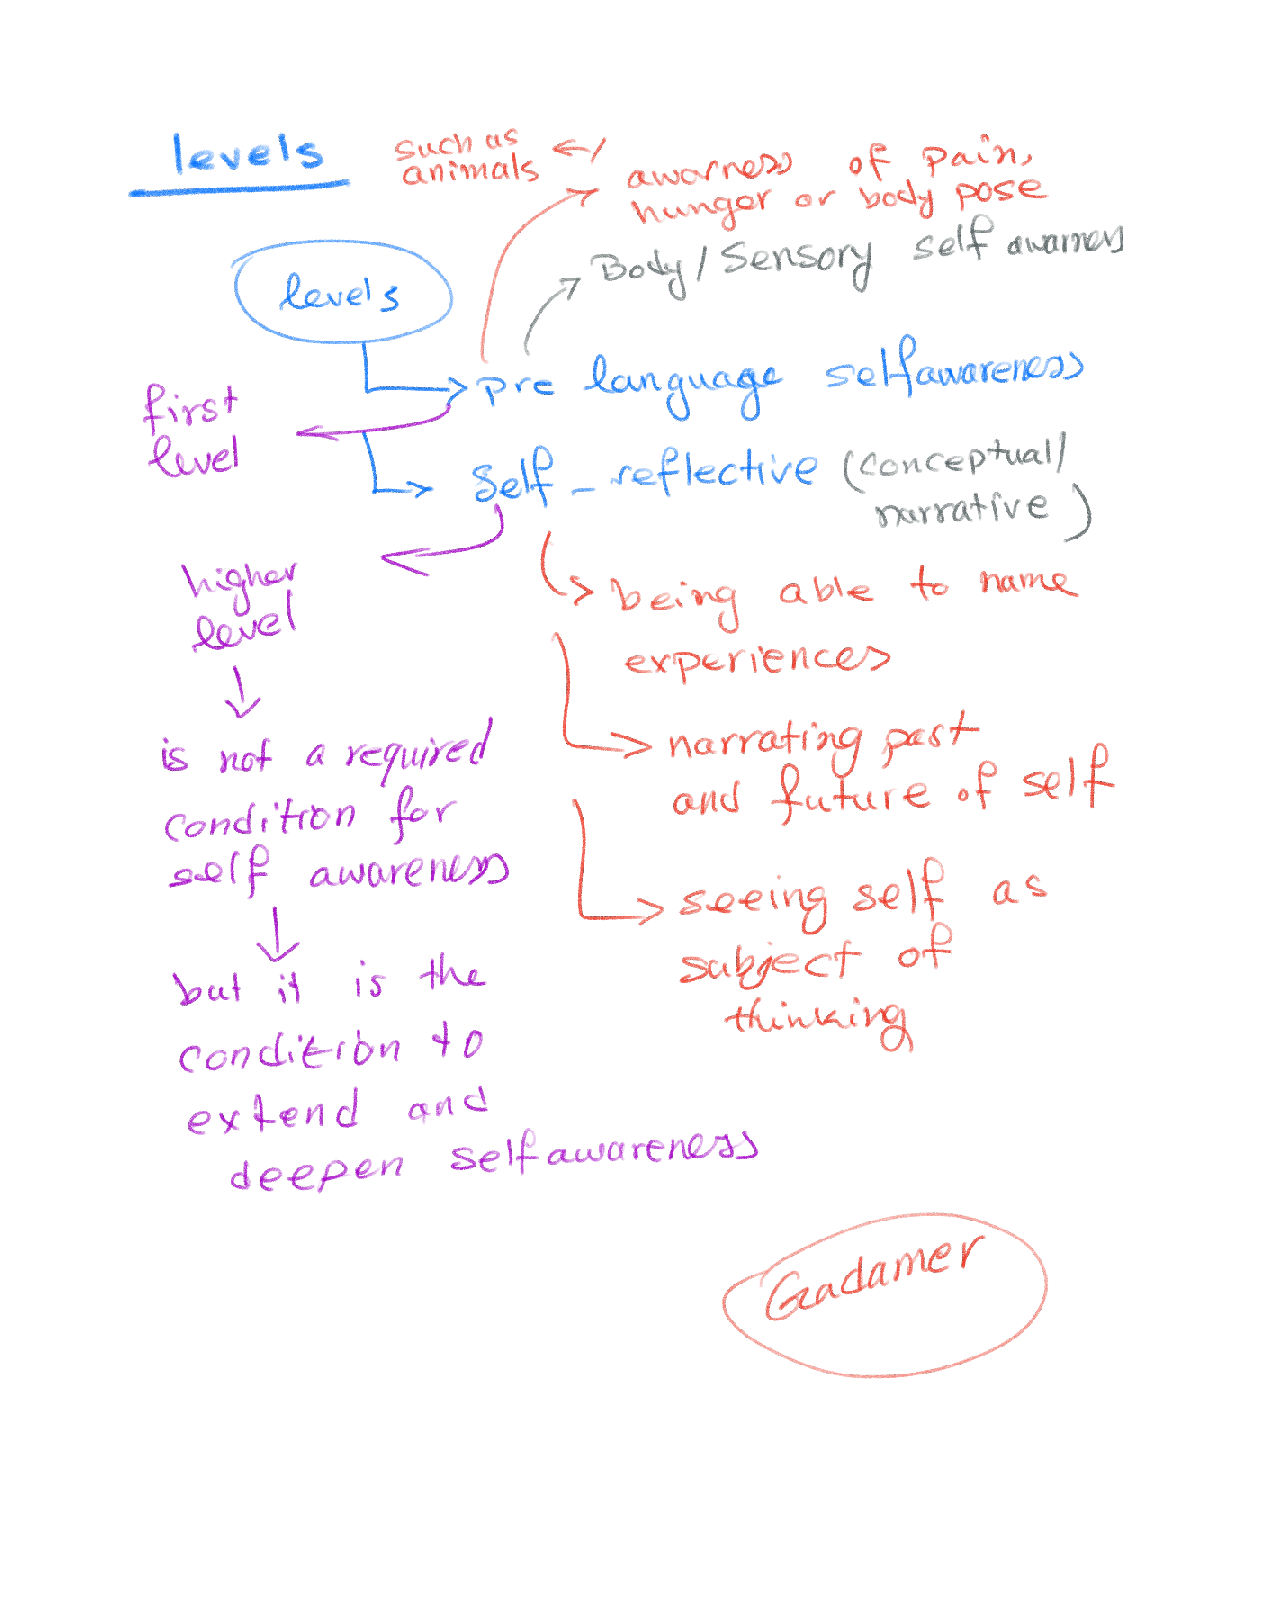
\includepdf[pages=-]{/home/donkarlo/Dropbox/repo/robotic_learning_project/figs/self_awareness.pdf}
    
    